\documentclass[11pt,aspectratio=169]{beamer}
\usetheme{Boadilla}
\usecolortheme{seagull}
\setbeamertemplate{navigation symbols}{}
\setbeamertemplate{footline}[frame number]
\setbeamercolor{title}{fg=black}
\setbeamercolor{frametitle}{fg=black,bg=white}
\setbeamerfont{frametitle}{series=\bfseries}

\usepackage{graphicx}
\usepackage{booktabs}
\usepackage{amsmath}

\title{Probabilistic dengue and chikungunya forecasting in Brazil}
\subtitle{Team Neural Earth --- Methodology, IMDC 2026}
\author{Md Kamruzzaman Kamrul \and Eashraque Jahan Easha \and Abdullah Al Helal}
\institute{Purdue University \and University of Denver \and Oklahoma State University}
\date{Internal methodology webinar, 22 September 2026}

\begin{document}

\begin{frame}
\titlepage
\end{frame}

% ---------------------------------------------------------------
\begin{frame}{The problem}
\begin{itemize}
  \item Brazil's 2024 dengue season broke the national record by roughly 4$\times$: 451{,}578
        cases in a single epidemiological week, $\sim$6.67M for the year.
  \item Preparedness needs \textbf{calibrated probabilistic forecasts}, not point estimates:
        the full range of plausible outcomes, not just an expected value.
  \item Open question this challenge exposes: which modeling paradigm (statistical, ML, DL,
        mechanistic) forecasts best, and how robustly, when a season can depart by an order of
        magnitude from the training record?
\end{itemize}
\vfill
\textbf{Our approach:} one leakage-safe backtesting harness, five model families, evaluated
identically across four official seasons and 26 mandatory states, combined into a
conformally-recalibrated ensemble.
\end{frame}

% ---------------------------------------------------------------
\begin{frame}{Study design}
\centering
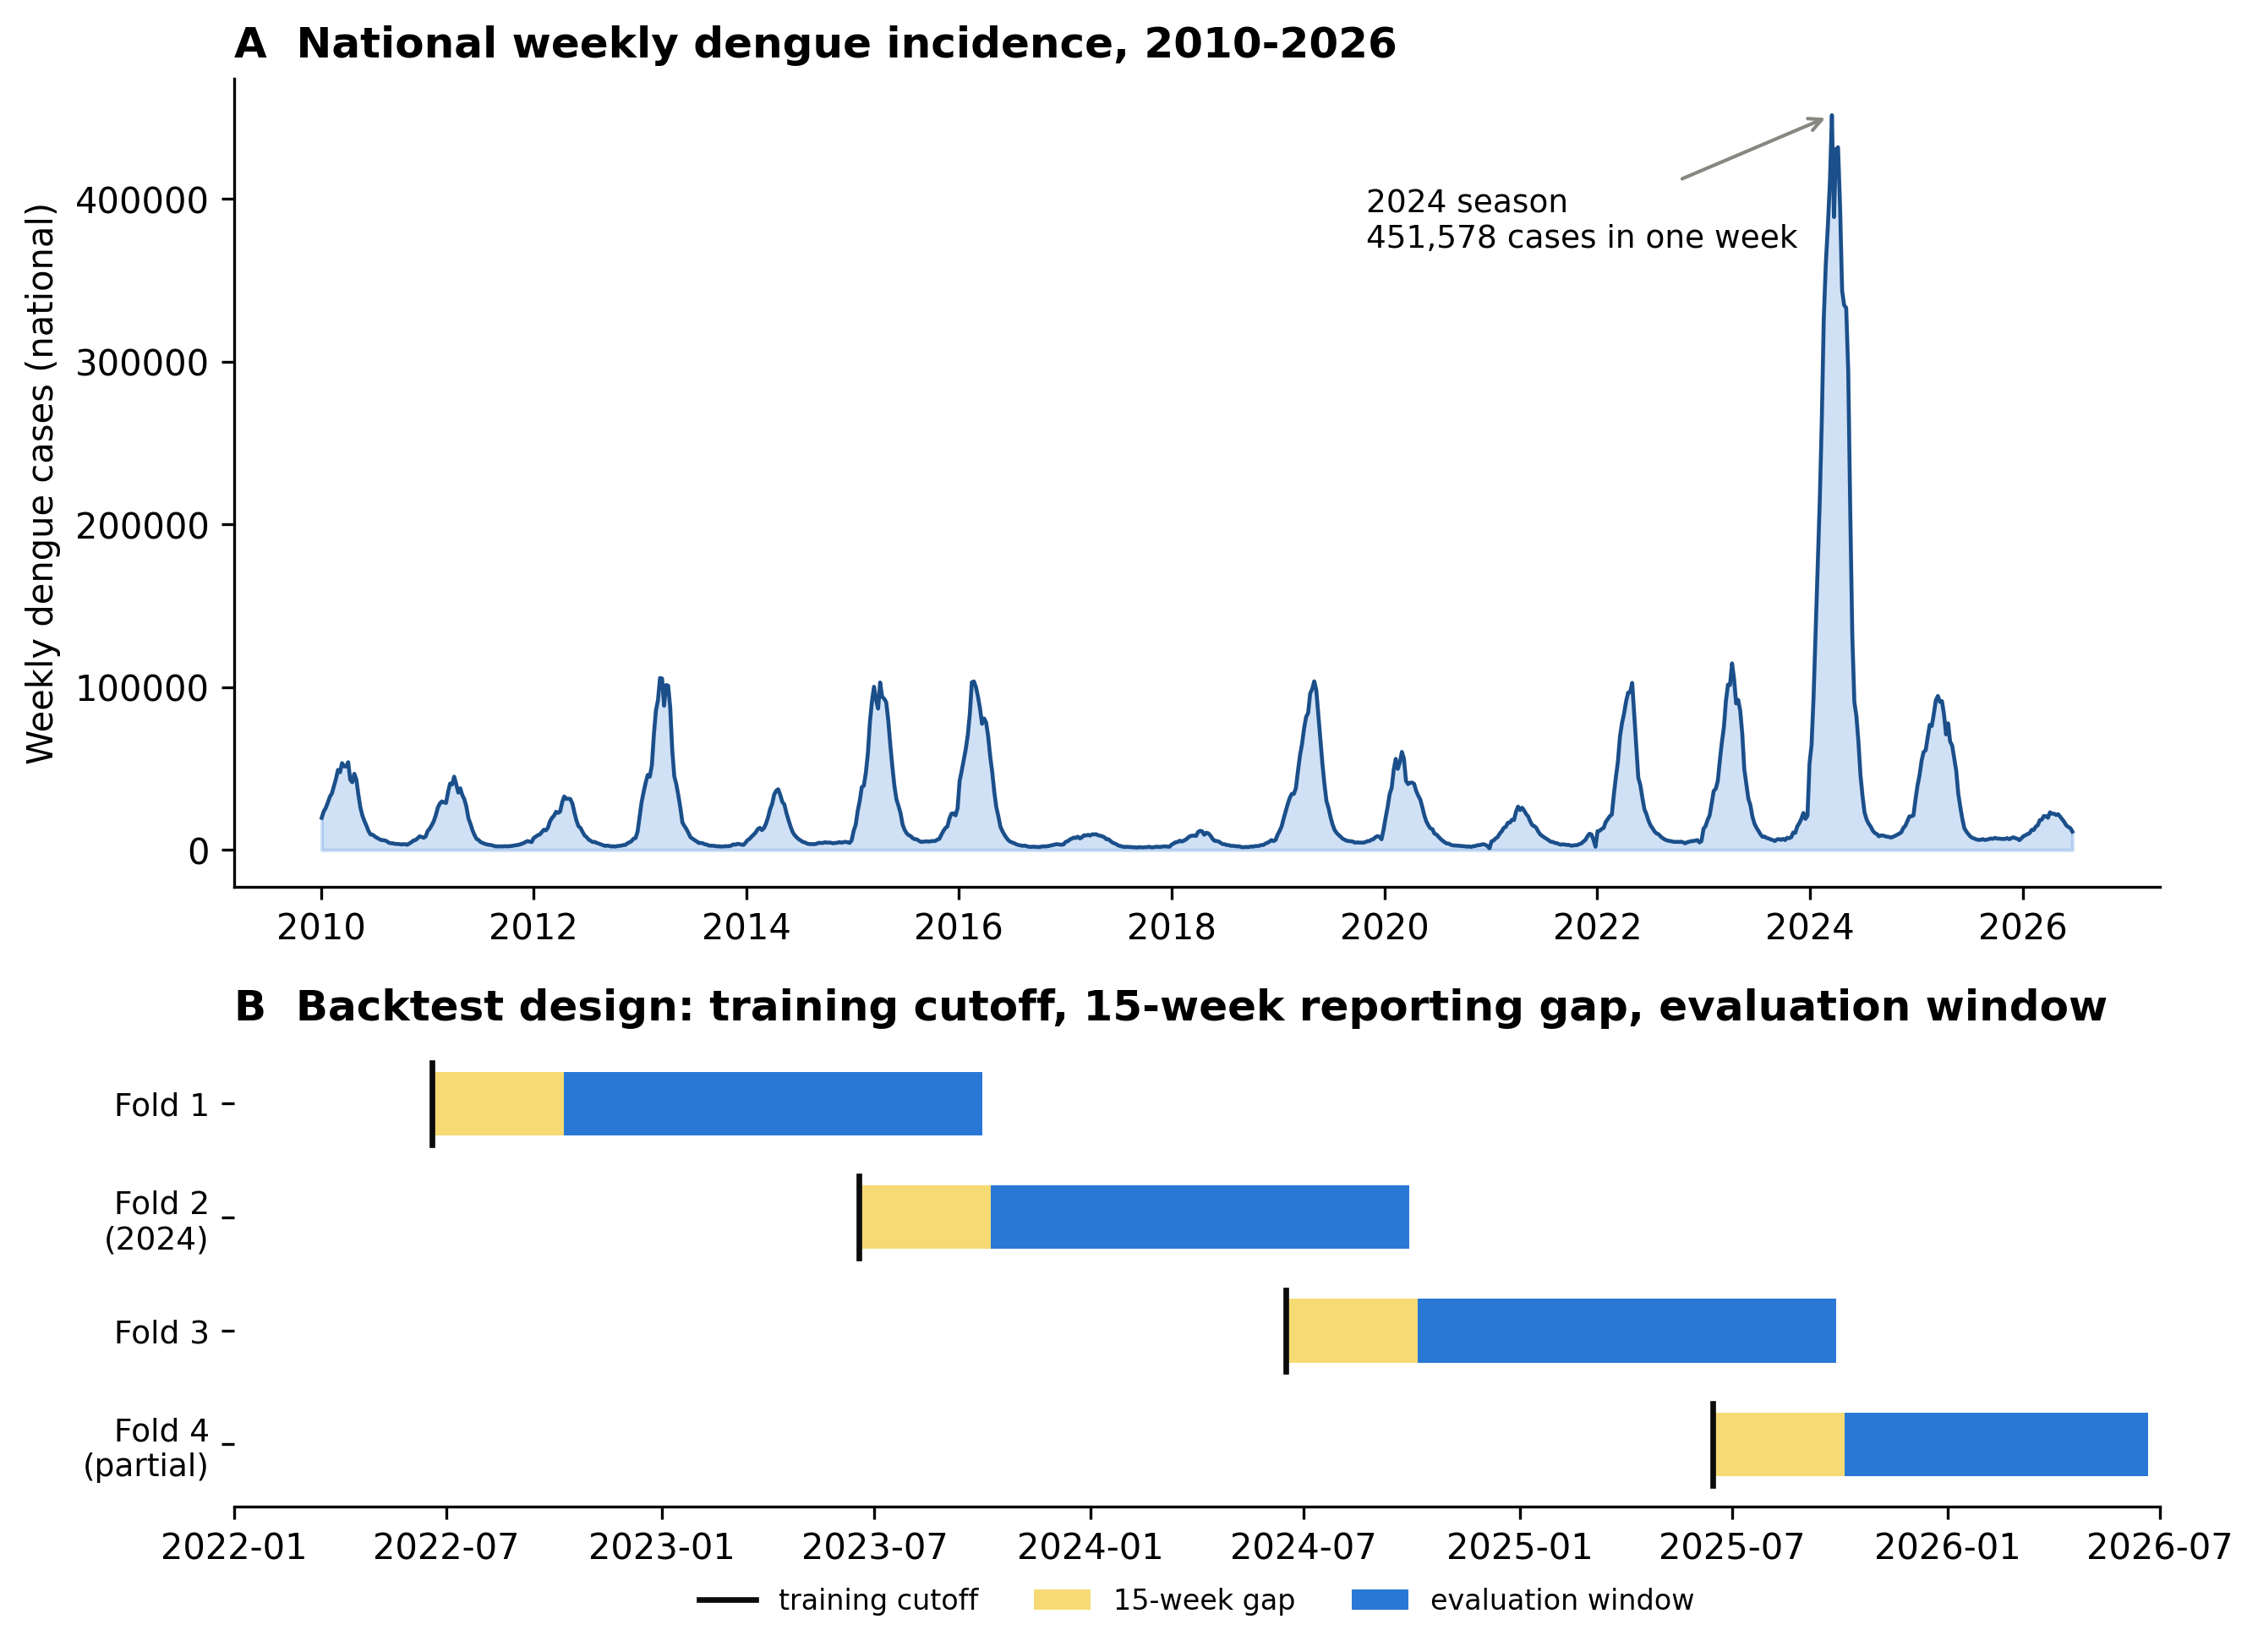
\includegraphics[width=0.68\textwidth]{../results/figures/paper_design.png}
\end{frame}

% ---------------------------------------------------------------
\begin{frame}{Leakage-safe backtest discipline}
\begin{itemize}
  \item Fold boundaries derived at runtime from the challenge's own \texttt{train\_N}/\texttt{target\_N}
        flags --- never hardcoded, so the pipeline stays correct if the data is refreshed.
  \item A confirmed \textbf{15-week reporting gap} sits between each fold's training cutoff and its
        target window in every official fold. Every joined covariate table (climate, ocean indices,
        search-access) is explicitly date-filtered to the cutoff, not inferred from the target flag,
        so this gap cannot leak into training.
  \item The ECMWF seasonal-forecast product is filtered by \emph{issue date}, not target date: a
        legitimate future covariate only if it was issued on or before the cutoff.
  \item A hard leakage assertion guards the whole pipeline, backed by dedicated regression tests.
  \item Same machinery, unchanged, produces the real forecast-phase submission
        (train cutoff = EW25 2026, target EW41 2026 $\to$ EW40 2027).
\end{itemize}
\end{frame}

% ---------------------------------------------------------------
\begin{frame}{Five model families, one harness}
\begin{itemize}
  \item \textbf{Baselines} --- naive, seasonal-naive, climatological quantile (empirical
        same-epiweek quantiles).
  \item \textbf{LightGBM} --- quantile regression on a synthetic-origin panel (weekly origins
        $\times$ horizons 1--67), direct multi-horizon, with conformalized quantile regression
        (CQR) calibration.
  \item \textbf{GRU} --- global recurrent network, per-state embeddings, negative-binomial head,
        5-member deep ensemble.
  \item \textbf{Mechanistic} --- Richards-curve bootstrap of historical trajectories with a
        negative-binomial observation model; intervals widen with historical variability by
        construction.
  \item \textbf{Ensemble} --- per-quantile median (Vincentization) of climatological + LightGBM +
        GRU, then conformal recalibration of the tails.
\end{itemize}
\end{frame}

% ---------------------------------------------------------------
\begin{frame}{Finding 1: no single model dominates}
\centering
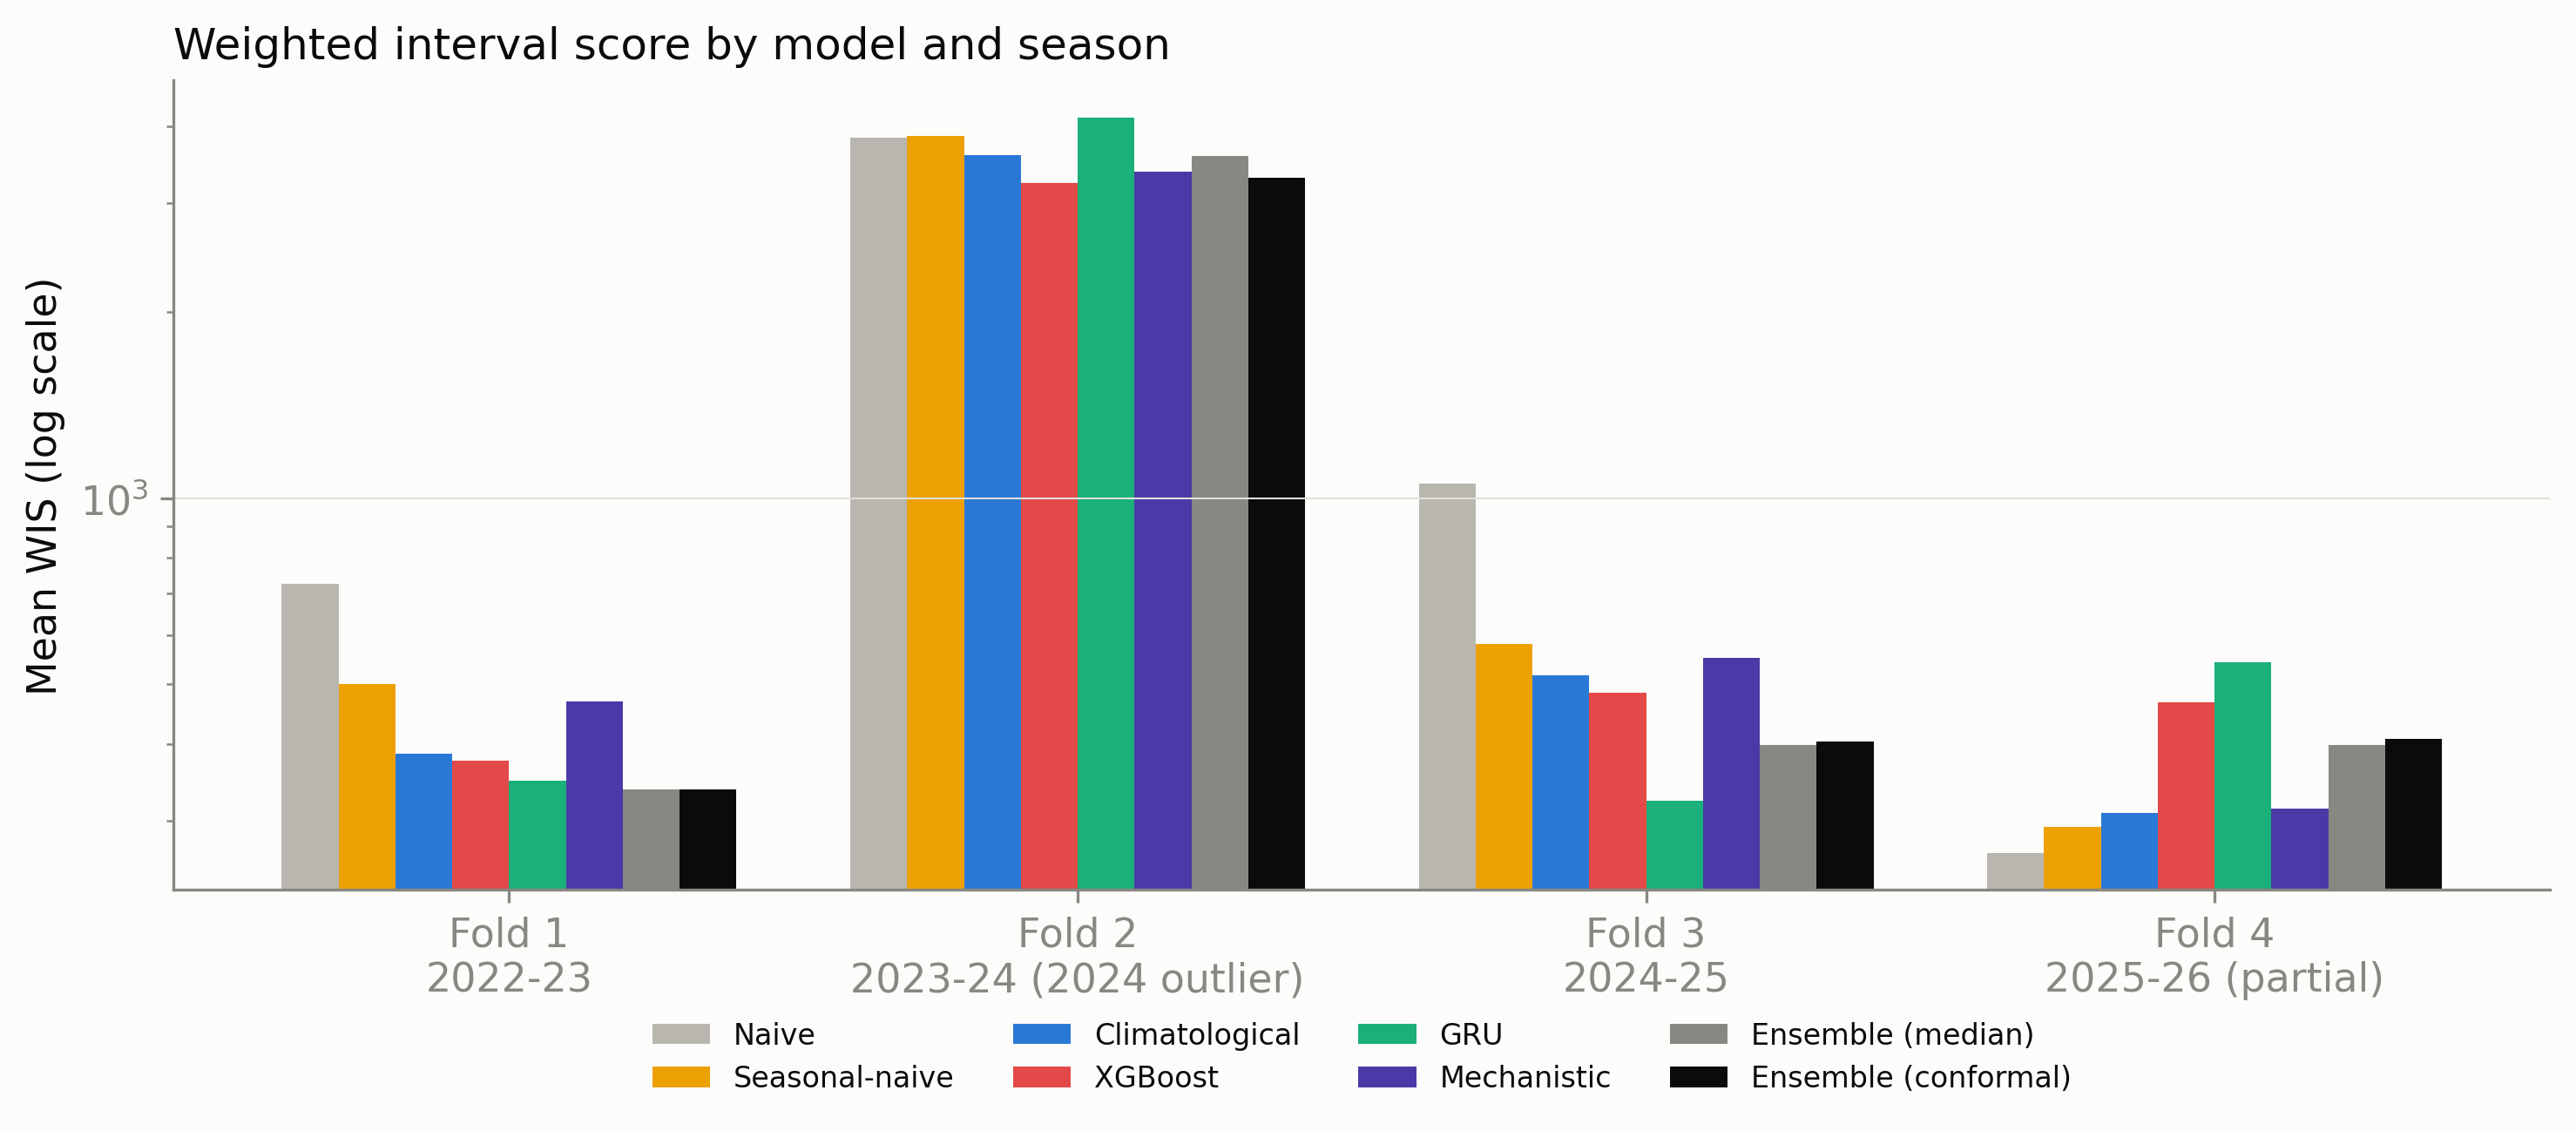
\includegraphics[width=0.72\textwidth]{../results/figures/paper_wis_by_fold.png}
\vfill
\small The GRU is best in ordinary seasons, worst on the 2024 outlier. LightGBM shows the
opposite profile. The ensemble never suffers a member's worst-season failure.
\end{frame}

% ---------------------------------------------------------------
\begin{frame}{Skill and stability are different axes}
\centering
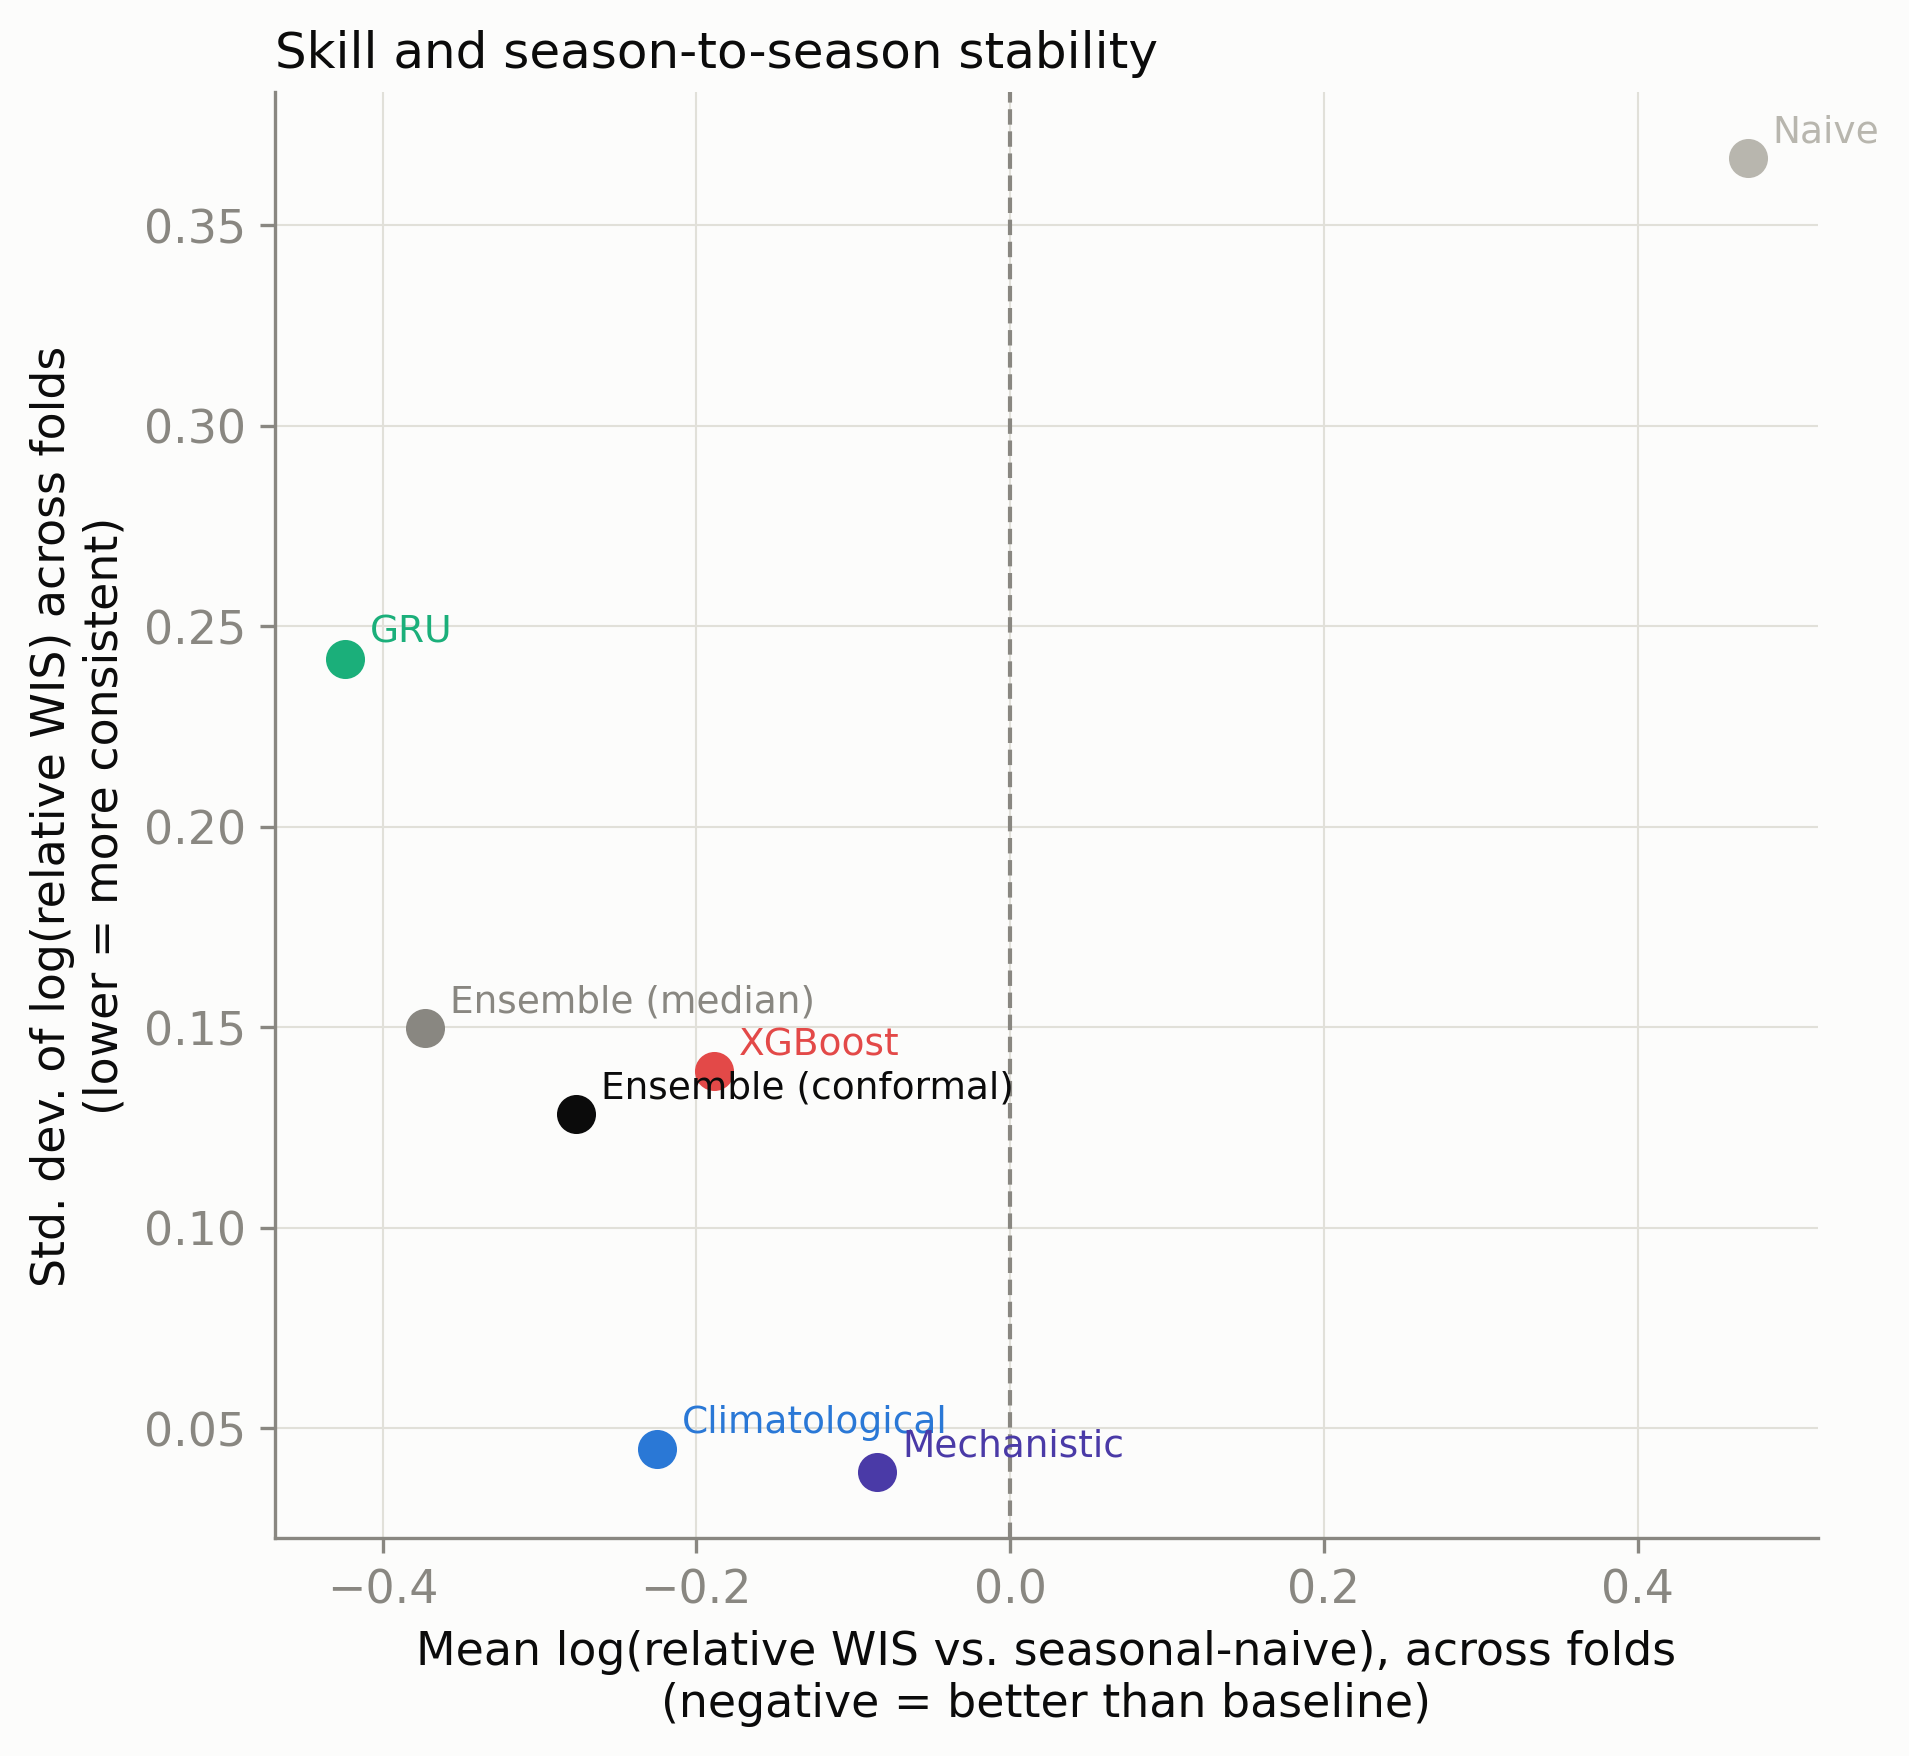
\includegraphics[width=0.42\textwidth]{../results/figures/paper_stability.png}
\vfill
\small Mean vs.\ std-dev of log relative WIS across folds. The GRU has the best mean skill but
is among the least stable; the mechanistic model is the most stable but modest; the ensembles
occupy a position no single member reaches.
\end{frame}

% ---------------------------------------------------------------
\begin{frame}{Finding 2: conformal recalibration is cheap, transferable insurance}
\centering
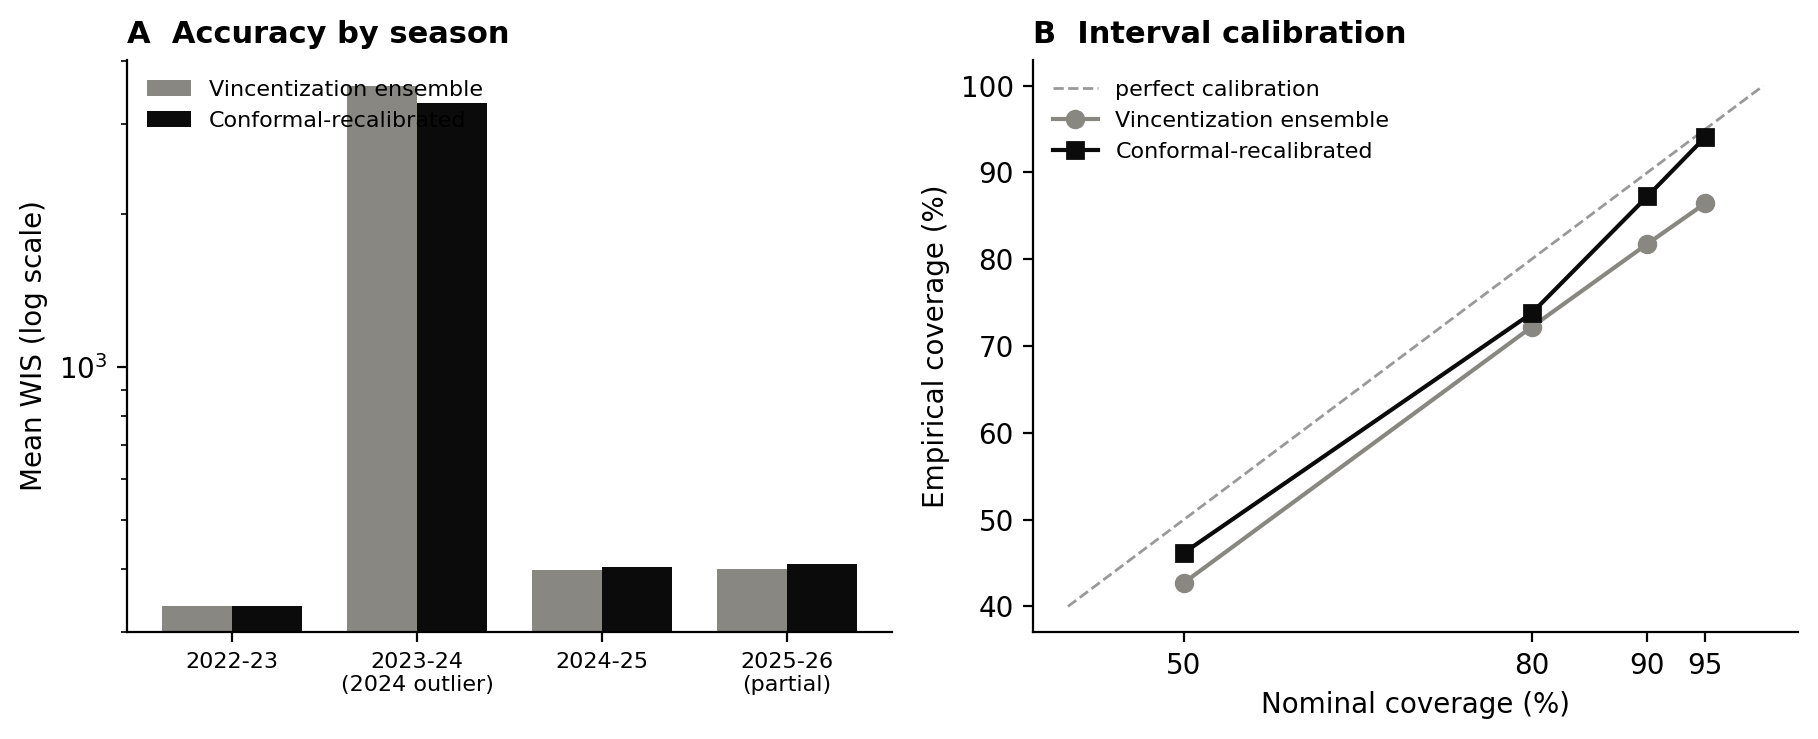
\includegraphics[width=0.92\textwidth]{../results/figures/paper_conformal.png}
\vfill
\small Factors \{50: 1.03, 80: 1.00, 90: 1.23, 95: 1.73\} tuned on one season, applied to all
others. Mean WIS 1281 $\to$ 1216 (out-of-sample $-5.5\%$); coverage 46/76/84/88 $\to$ 47/76/88/93.
Gain concentrates in the outbreak season at negligible cost elsewhere.
\end{frame}

% ---------------------------------------------------------------
\begin{frame}{Finding 3: the winner depends on the metric}
\centering
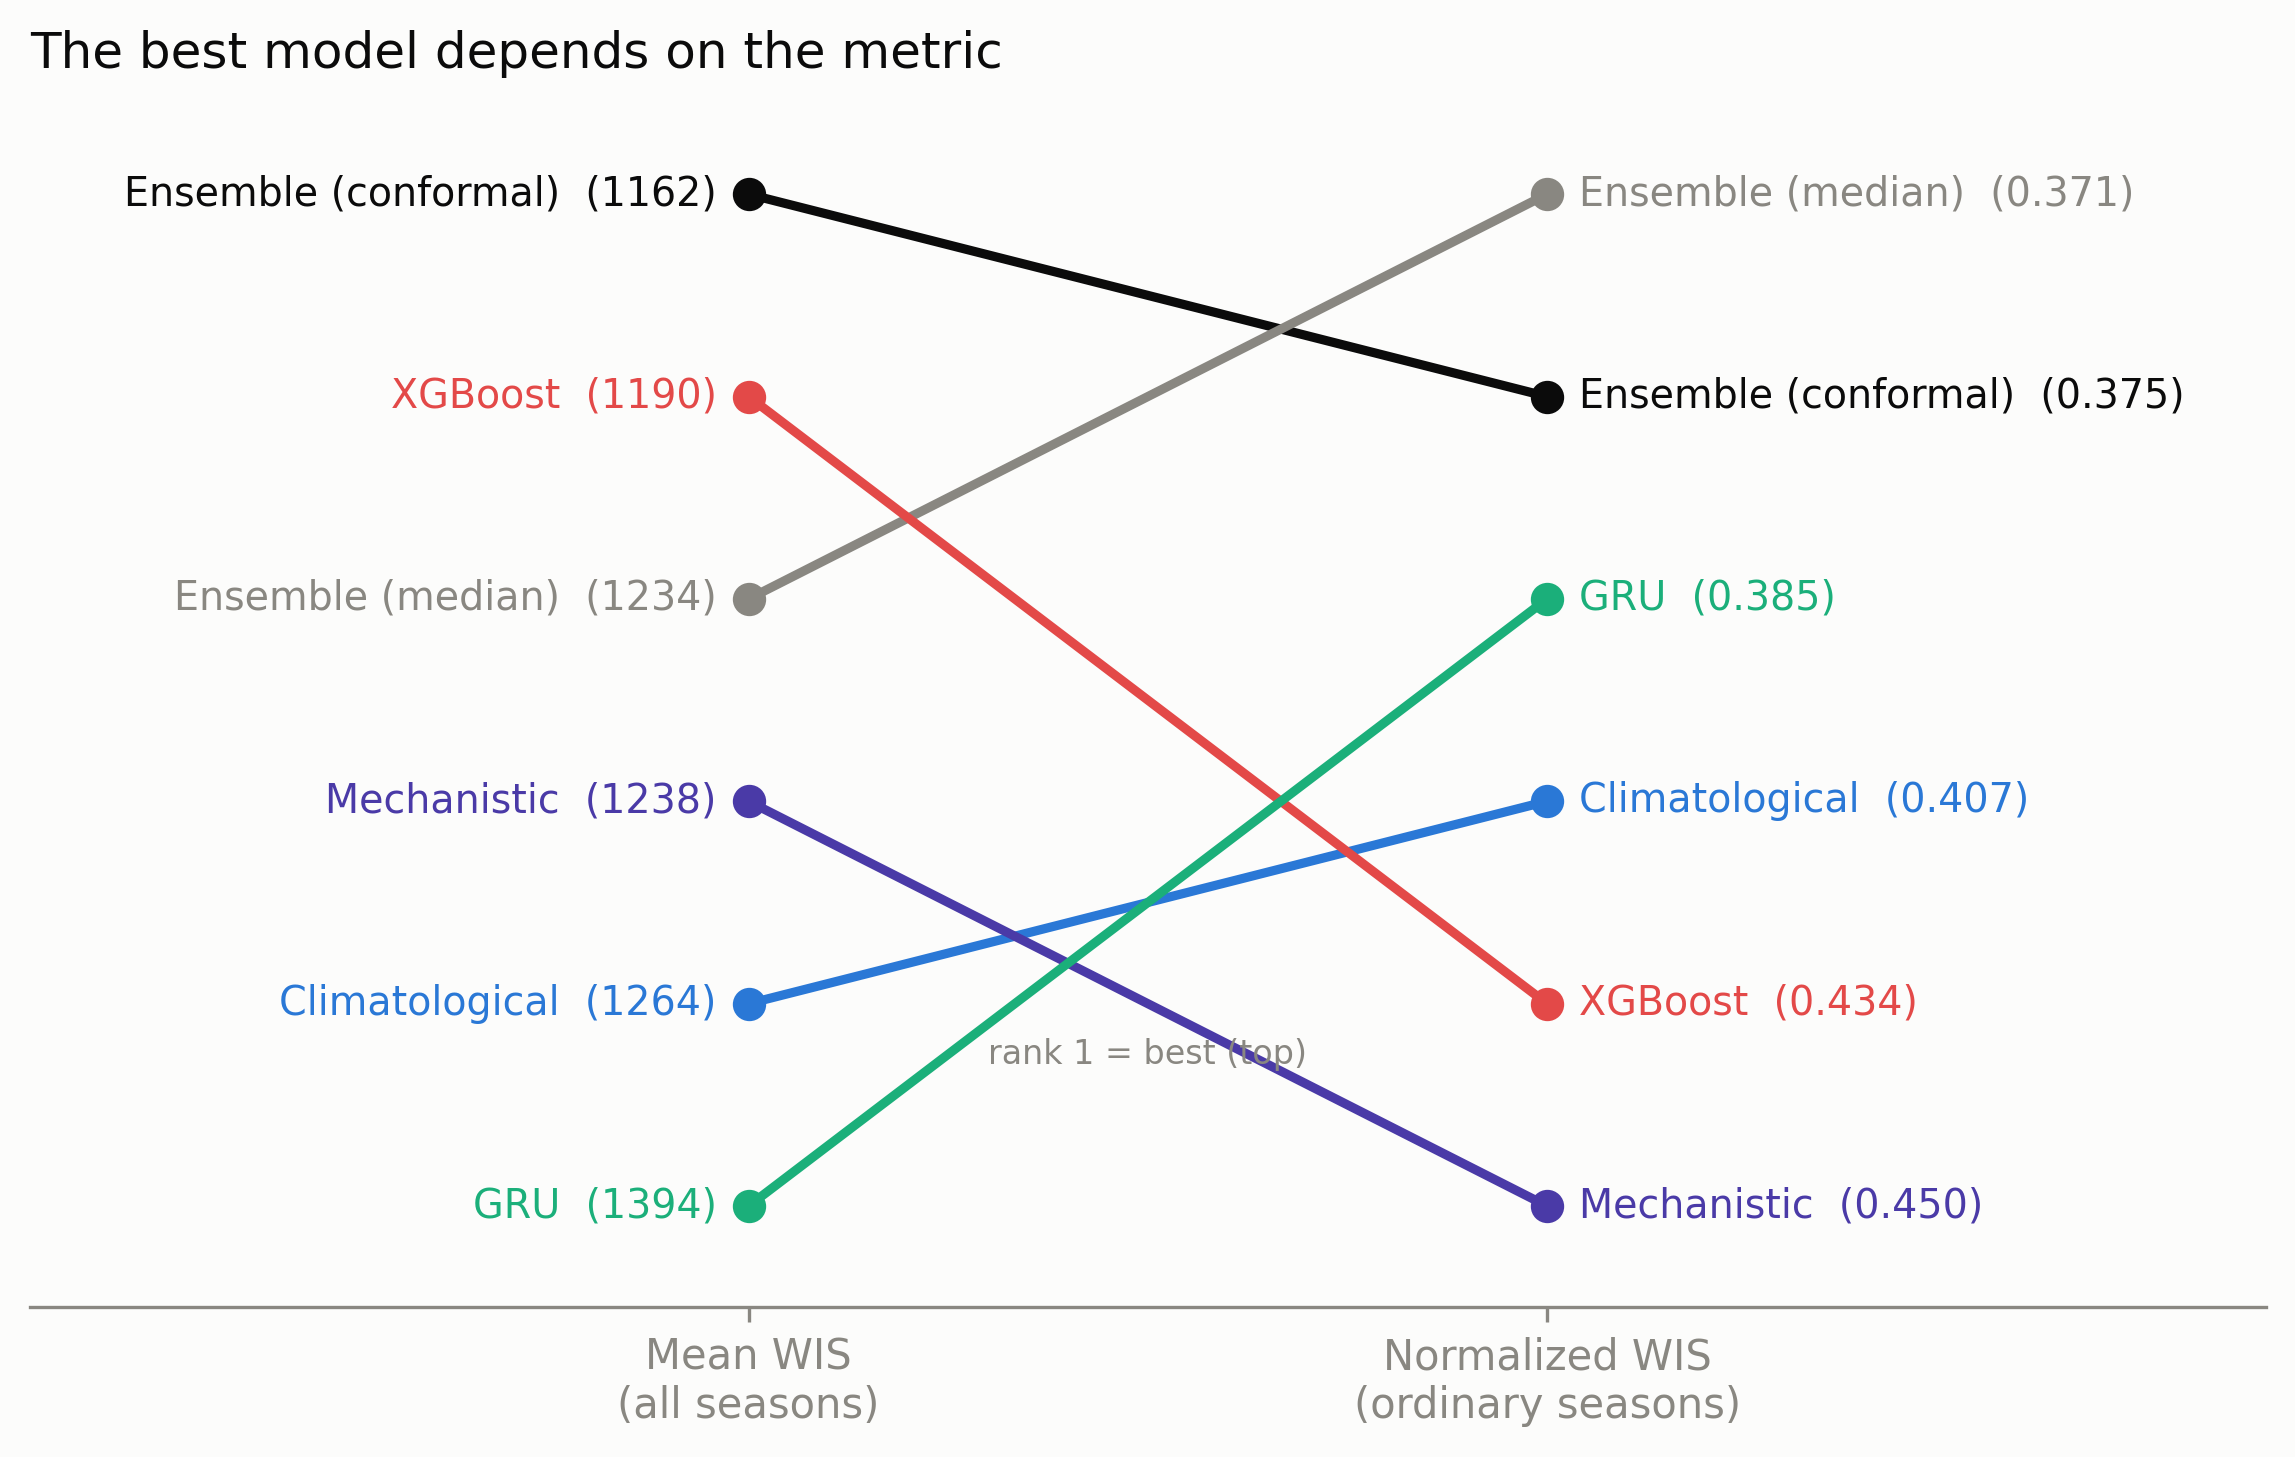
\includegraphics[width=0.62\textwidth]{../results/figures/paper_relative_wis.png}
\vfill
\small Magnitude-weighted mean WIS and scale-free normalized WIS reward accuracy on different
subsets of a highly skewed set of states. We report both; a single aggregate can mislead.
\end{frame}

% ---------------------------------------------------------------
\begin{frame}{Finding 4: added complexity did not pay}
\begin{itemize}
  \item \textbf{Observed climate covariates} added to LightGBM: WIS \textbf{worsened} (1299
        $\to$ 1342). The forecast-relevant signal is the ECMWF seasonal forecast and ENSO, not
        observed weather --- observed climate is already implicit in recent case lags.
  \item \textbf{Hierarchical macroregion pooling} of seasonal climatology: WIS worsened (1216
        $\to$ 1241). States are too heterogeneous within a macroregion for naive pooling to help.
  \item An internal-holdout hyperparameter search that \emph{improved} the holdout
        \emph{worsened} the true backtest --- a caution about tuning discipline in
        heavily-autocorrelated synthetic-origin panels.
  \item Simple methods (climatological quantile, a historical-trajectory bootstrap) are hard to
        beat, consistent with small-sample, few-series forecasting-competition evidence.
\end{itemize}
\end{frame}

% ---------------------------------------------------------------
\begin{frame}{Beyond the aggregate: per-state and disease-specific results}
\centering
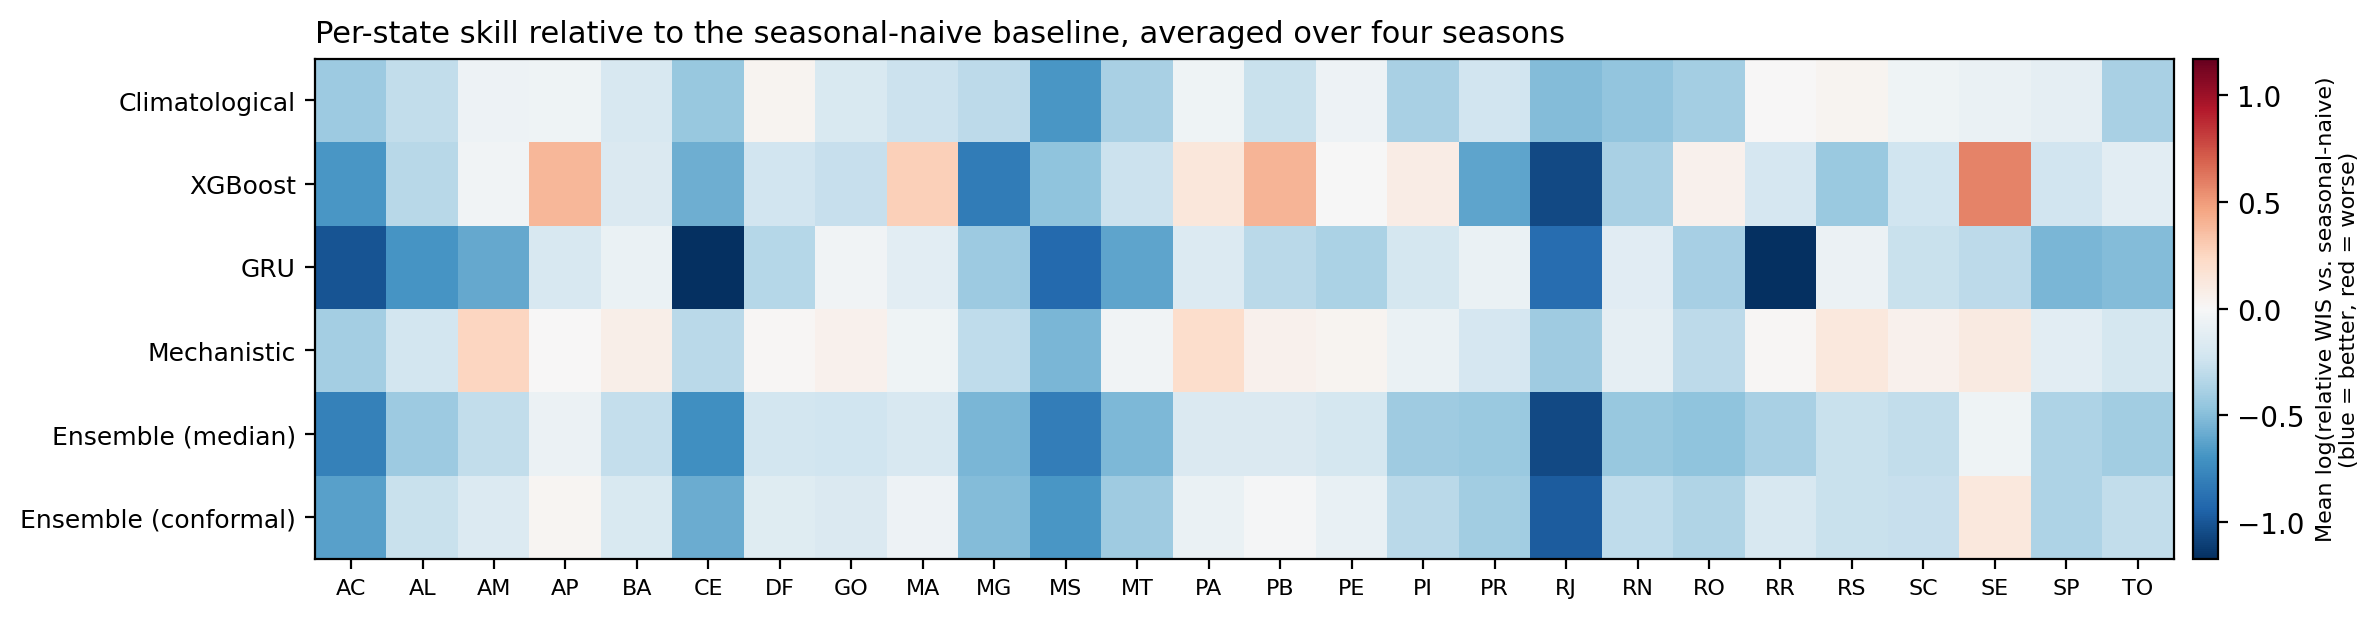
\includegraphics[width=\textwidth]{../results/figures/paper_state_heatmap.png}
\vfill
\small Per-state skill relative to the seasonal-naive baseline. The GRU's advantage
concentrates in specific states rather than being uniform. Chikungunya: gradient boosting alone
beats the ensemble (WIS 82.3 vs.\ 91.6) --- the best model is disease-specific.
\end{frame}

% ---------------------------------------------------------------
\begin{frame}{Independent recognition and current status}
\begin{itemize}
  \item At the 31 July 2026 validation-round webinar, our submission was named:
  \begin{itemize}
    \item one of \textbf{6 best-overall-performing models} (of 27) for the mandatory dengue
          state-level target;
    \item one of \textbf{3 models with outstanding performance} on the optional city-level
          target.
  \end{itemize}
  \item \textbf{Forecast phase (2026--27 season) submitted} 6 September 2026, ahead of the
        10 September deadline, using the same harness and the conformal-recalibrated ensemble.
  \item Public repository: leakage tests, scoring-correctness tests, determinism guards,
        provenance manifest, and validated submissions for all four official tracks.
\end{itemize}
\end{frame}

% ---------------------------------------------------------------
\begin{frame}{Takeaways}
\begin{enumerate}
  \item Model rankings are season-dependent; a model chosen on average performance can be the
        least reliable exactly when an outbreak makes accuracy matter most.
  \item An unweighted ensemble is never the single worst model in any season, and conformal
        recalibration turns it into the single best, at negligible cost.
  \item Metric choice is a reporting-standards issue, not a modeling one: report both
        magnitude-weighted and scale-free skill.
  \item Complexity did not pay here: the signal that helps is the \emph{right} covariate
        (seasonal forecast, not observed weather), not more of it.
\end{enumerate}
\vfill
\centering \texttt{github.com/kamrul28890/3rd\_imdc\_purdue\_neuralearth}
\end{frame}

\end{document}
